\chapter{RESULTS AND DISCUSSION} 
\section{ECG Monitoring Through Ubidots}
The project successfully implements the AD8232 sensor for ECG signal analysis. Data is sent to an IoT platform, allowing easy at-home heart rate monitoring for patients. Healthcare providers can remotely assess heart health through the platform. The project aims for a user-friendly system, emphasizing real-time data transmission. The circuit diagram illustrates the sensor's integration for efficient ECG analysis \cite{vamseekrishna2023low}
\\
The AD8232 sensor, crucial for this monitoring system, features nine connection points that allow for soldering pins, wires, or other connectors. Among these, the LO+, LO-, OUTPUT, SDN, 3.3V, and GND pins are essential for operation alongside the Nodemcu ESP8266 microcontroller, enabling data transmission and reception. Specifically, five general pins must be connected to the microcontroller: the output links to analog pin A0 of the Nodemcu\cite{sutikno2021internet}, while LO- and LO+ are attached to pins D6 and D5, respectively. Finally, the sensor is powered by connecting the supply pin to 3.3V and grounding the device for proper functionality within the monitoring setup.
 \begin{figure}[htbp]
    \centering
     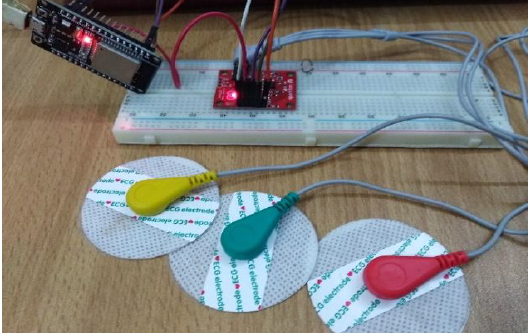
\includegraphics[width=0.6\linewidth]{C_chap/fig38.png}
\\\caption{Prototype of Project}
 \end{figure}
\pagebreak
\\
As shown in Figure 4.2, the data is published into the Ubidots, and it is viewed in serial monitor once the MQTT connection is secured and connects successfully.
 \begin{figure}[htbp]
    \centering
     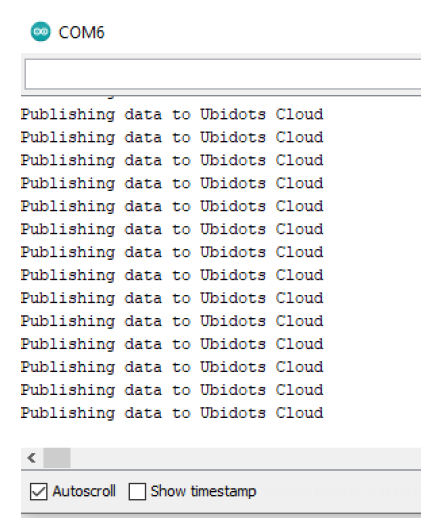
\includegraphics[width=0.6\linewidth]{C_chap/fig10.png}
\\\caption{The publishing of data into Ubidots}
 \end{figure}
\\
The process of ECG signal analysis involves identifying specific points within the ECG waveform to understand the heart's electrical activity. The R-peak, which represents the peak of the QRS complex, is a crucial point in the ECG signal. It signifies the ventricular depolarization, the moment when the main pumping chambers of the heart contract to push blood out. The R-peak is recognized as the highest point in each cycle of the ECG waveform, and it serves as a key reference point for analyzing heart rate and rhythm.
The QRS complex, comprising the Q, R, and S waves, provides important information about the electrical conduction through the ventricles. The span of the QRS complex is determined from the trigger point before the R-peak to the one after it. The Q wave represents the initial downward deflection, the R wave is the main upward deflection, and the S wave follows the R wave as a downward deflection. These waves collectively show the spread of electrical impulses across the ventricles, leading to their contraction.
Additionally, the T and S waves are crucial components of the ECG waveform. The T wave represents the repolarization of the ventricles, the moment when they relax and prepare for the next heartbeat. It is located after the QRS complex, usually in the upward direction. The S wave, on the other hand, is the downward deflection immediately following the R wave, indicating the end of ventricular depolarization.
"Real-time data" in this context refers to the immediate processing and display of ECG information for quick user response. In this system, as soon as the ECG signals are captured and analyzed, the results are presented to the user without delay. This allows for continuous and up-to-date monitoring of the heart's electrical activity, providing timely insights into heart rate, rhythm, and potential abnormalities. Healthcare providers can promptly assess the ECG data, make informed decisions, and intervene if necessary for effective heart health management. The system's ability to offer continuous, real-time data presentation ensures that any changes or irregularities in the ECG signals can be promptly detected and addressed, enhancing patient care and monitoring.
 \begin{figure}[htbp]
    \centering
     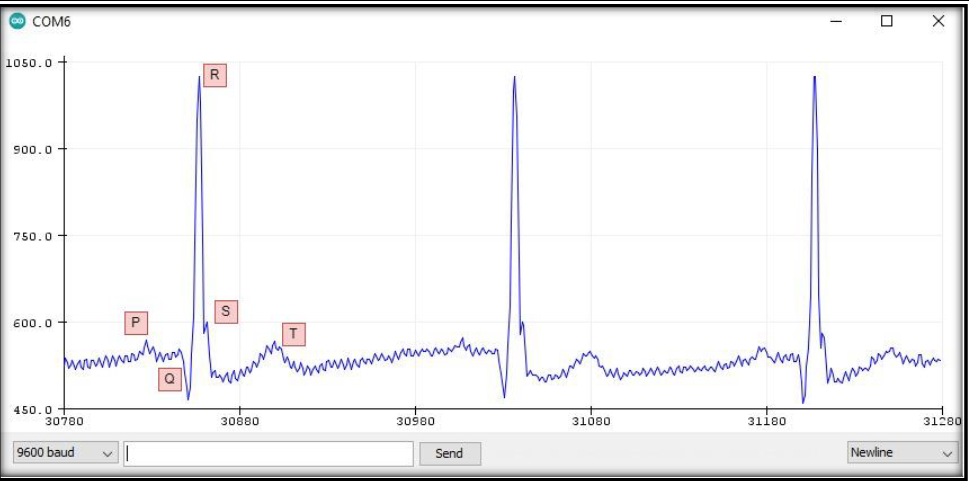
\includegraphics[width=0.9\linewidth]{C_chap/fig11.png}
\\\caption{The Signal in Serial Monitor}
 \end{figure}
\\
The dashboard of Ubidots, as depicted in Figure 4.4, serves as a visual representation of the heart signals captured and analyzed from the sensor data. Here, users can observe the ECG signals generated from the heart of subject 1, showcasing the characteristic waves of P, Q, R, S, and T in their normal, steady-state positions. Each of these waves corresponds to a specific phase of the cardiac cycle, providing valuable insights into the heart's electrical activity \cite{kleiman2021comparison}.
\begin{itemize}
    \item The P wave represents the atrial depolarization, the contraction of the atria to push blood into the ventricles.
\end{itemize}
\begin{itemize}
    \item The QRS complex, consisting of the Q, R, and S waves, signifies the ventricular depolarization, the contraction of the main pumping chambers of the heart.
\end{itemize}
\begin{itemize}
    \item The T wave reflects the ventricular repolarization, the relaxation and resetting of the ventricles for the next heartbeat.
\end{itemize}
Interpreting these waves is crucial as it allows healthcare providers to understand the heart's rhythm, rate, and overall function. An ECG tracing can reveal if the heart is beating too slowly (bradycardia), too fast (tachycardia), or irregularly (arrhythmia). This information is vital for diagnosing various cardiac conditions, monitoring treatment effectiveness, and identifying potential abnormalities.
Furthermore, the data transmitted to Ubidots can also be extracted and analyzed in Excel, providing a more detailed and ordered view of the ECG signals. Healthcare professionals can use this data to track trends over time, compare multiple recordings, and make informed decisions about patient care.
 \begin{figure}[htbp]
    \centering
     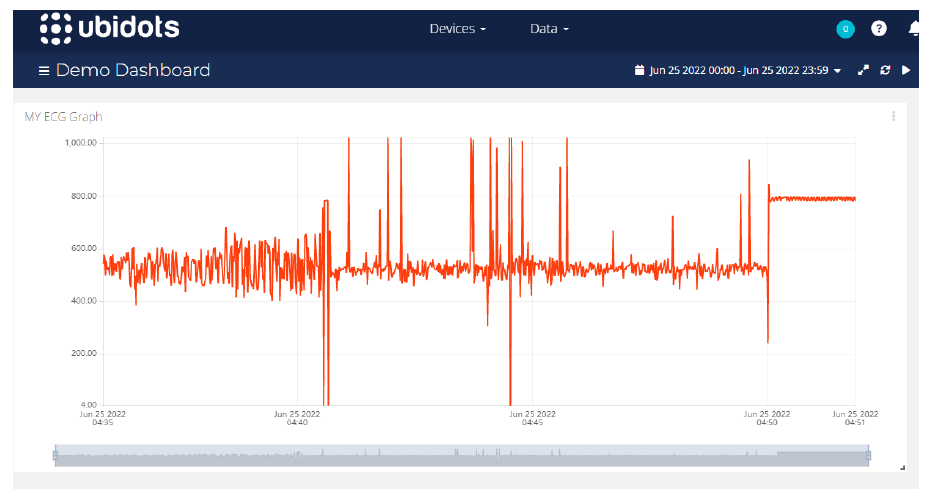
\includegraphics[width=0.9\linewidth]{C_chap/fig12.png}
\\\caption{Dashboard of Ubidots}
 \end{figure}
\pagebreak
\section{Depression Detection Through ML Model}
The machine learning model achieved an accuracy of 84\% on the training dataset and 77.34\% on the test dataset. This performance indicatesMore ECG data, often generated on the fly. However, the slight drop in accuracy from training to testing suggests that the model might be slightly providing training to the training data, meaning it may have learned to memorize patterns specific to the training set rather than capturing unspecified patterns. To address this, techniques such as regularization, data augmentation, or adjusting model complexity could be explored to improve the model's performance on unseen data. Additionally, further analysis of misclassified instances in the test set could provide insights into areas where the model struggles and guide further refinement efforts.\cite{chiong2021textual}
\\
 \begin{figure}[htbp]
    \centering
     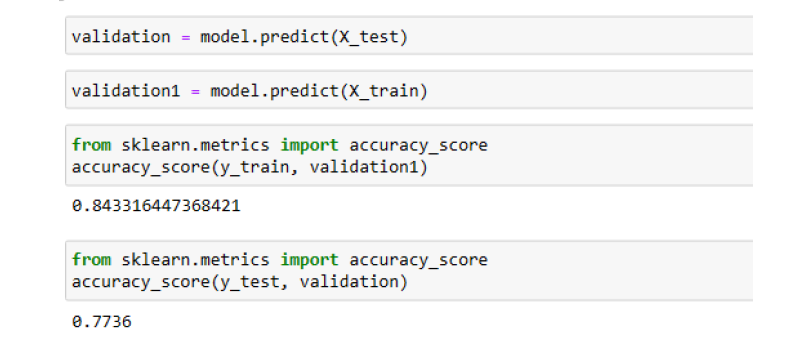
\includegraphics[width=0.9\linewidth]{C_chap/fig22.png}
\\\caption{Result of ML Model}
 \end{figure}
\\
In the realm of future research endeavors, the exploration of alternative machine learning and deep learning techniques stands poised as a promising avenue for enhancing prediction accuracy. Leveraging the expansive landscape of methodologies, including ensemble methods, convolution neural networks, and recurrent neural networks, holds the potential to unlock deeper insights and finer predictions. Furthermore, the acquisition of a comprehensive dataset, rich in diverse instances, presents an opportunity to fortify experimental endeavors. By amassing a wealth of data, researchers can delve into the nuances of complex patterns, thereby refining models to unprecedented levels of precision and robustness. This multifaceted approach not only promises to elevate predictive performance but also to push the boundaries of understanding within the field, fostering innovation and advancement.

 \begin{figure}[htbp]
    \centering
     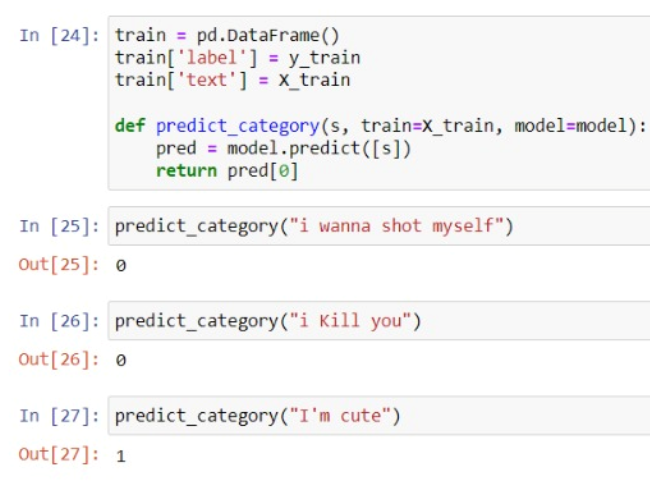
\includegraphics[width=0.8\linewidth]{C_chap/fig25.png}
\\\caption{Predictions of ML Model}
 \end{figure}

This project aimed to harness sentiment analysis as a tool for detecting depression, utilizing a dataset sourced from Kaggle. The dataset underwent meticulous processing and cleansing to ensure its readiness for analysis. Subsequently, the dataset was partitioned into 80 \% for training and 20 \% for testing purposes. Employing renowned machine learning algorithms, such as Naive Bayes, the experiments unfolded, yielding compelling results. Notably, the Naive Bayes technique emerged as a frontrunner, showcasing a classification accuracy exceeding 84 \%. This achievement underscores the efficacy of sentiment analysis in discerning indicators of depression, marking a significant stride in leveraging computational techniques for mental health assessment.
\\
 \begin{figure}[htbp]
    \centering
     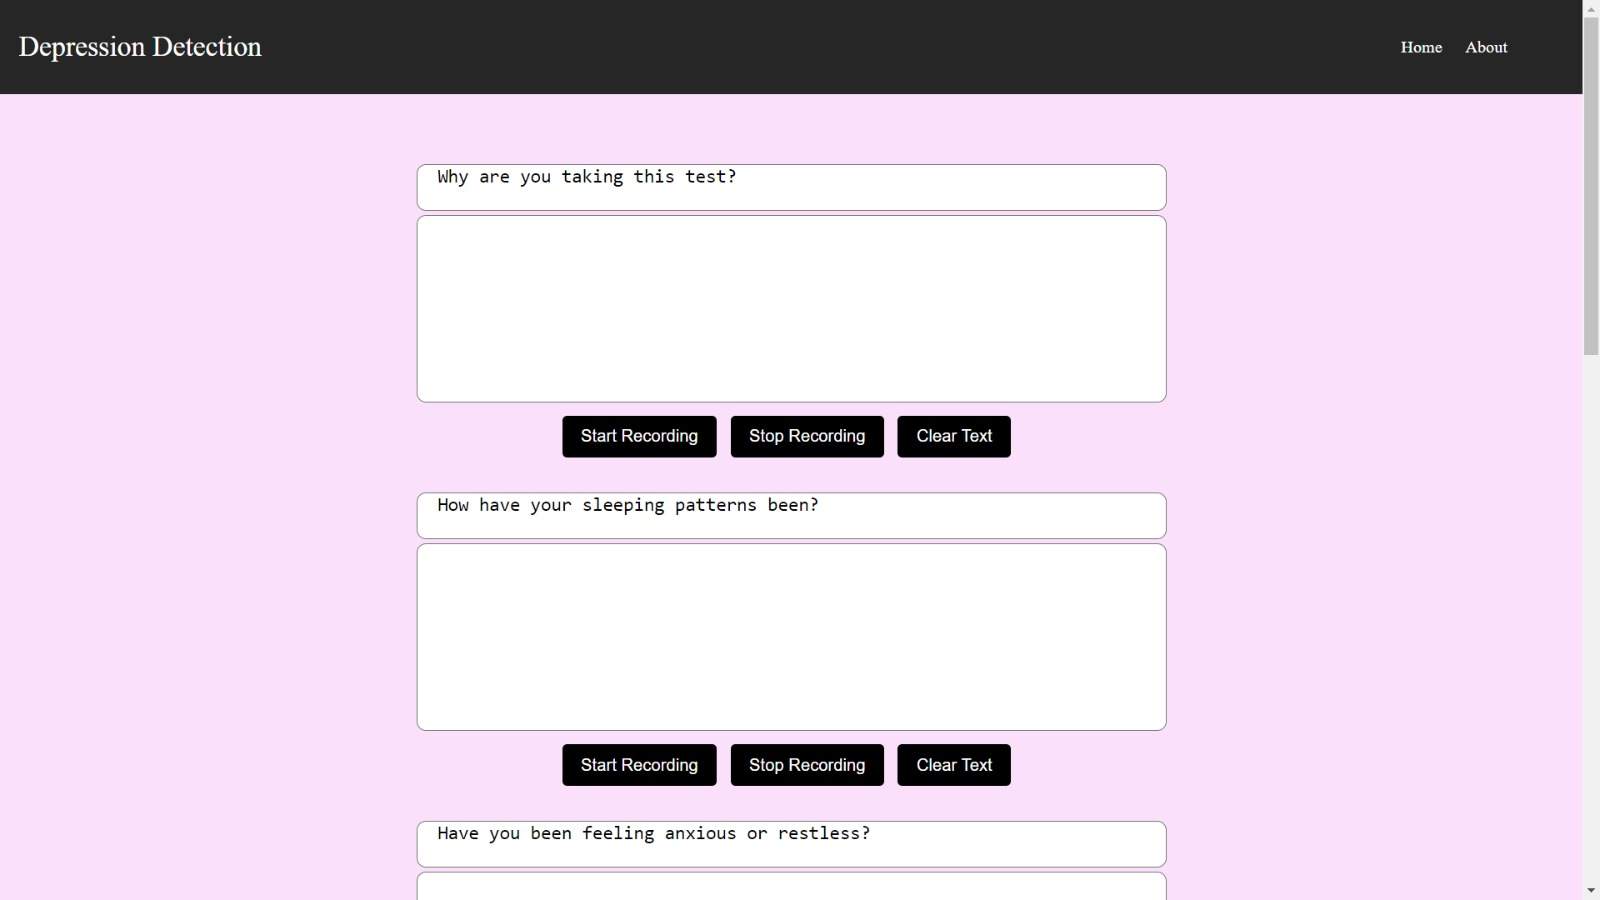
\includegraphics[width=1.0\linewidth]{C_chap/fig39.jpg}
\\\caption{Web Page of our Project}
 \end{figure}
 \begin{figure}[htbp]
    \centering
     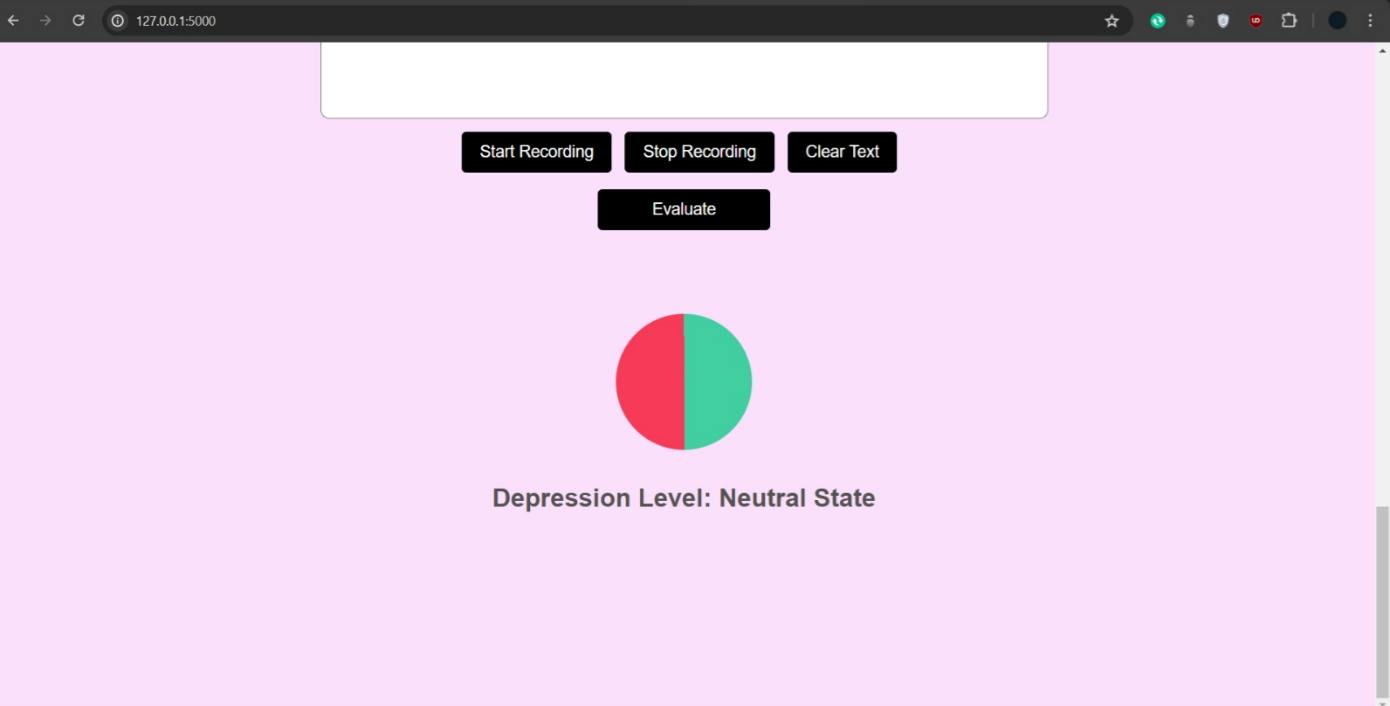
\includegraphics[width=1.0\linewidth]{C_chap/fig40.png}
\\\caption{Evaluation of Depression}
 \end{figure}
 \begin{figure}[htbp]
    \centering
     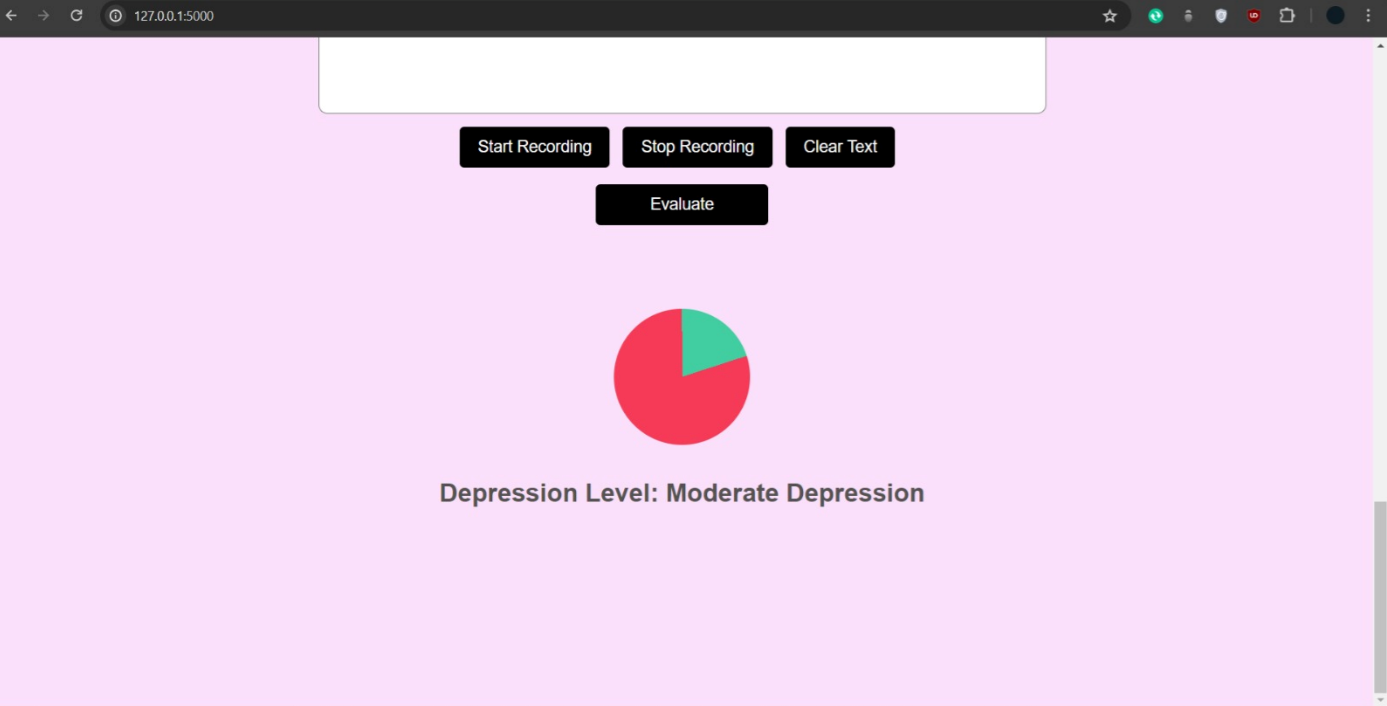
\includegraphics[width=1.0\linewidth]{C_chap/fig41.png}
\\\caption{Result of Depression Detection}
 \end{figure}
 \begin{figure}[htbp]
    \centering
     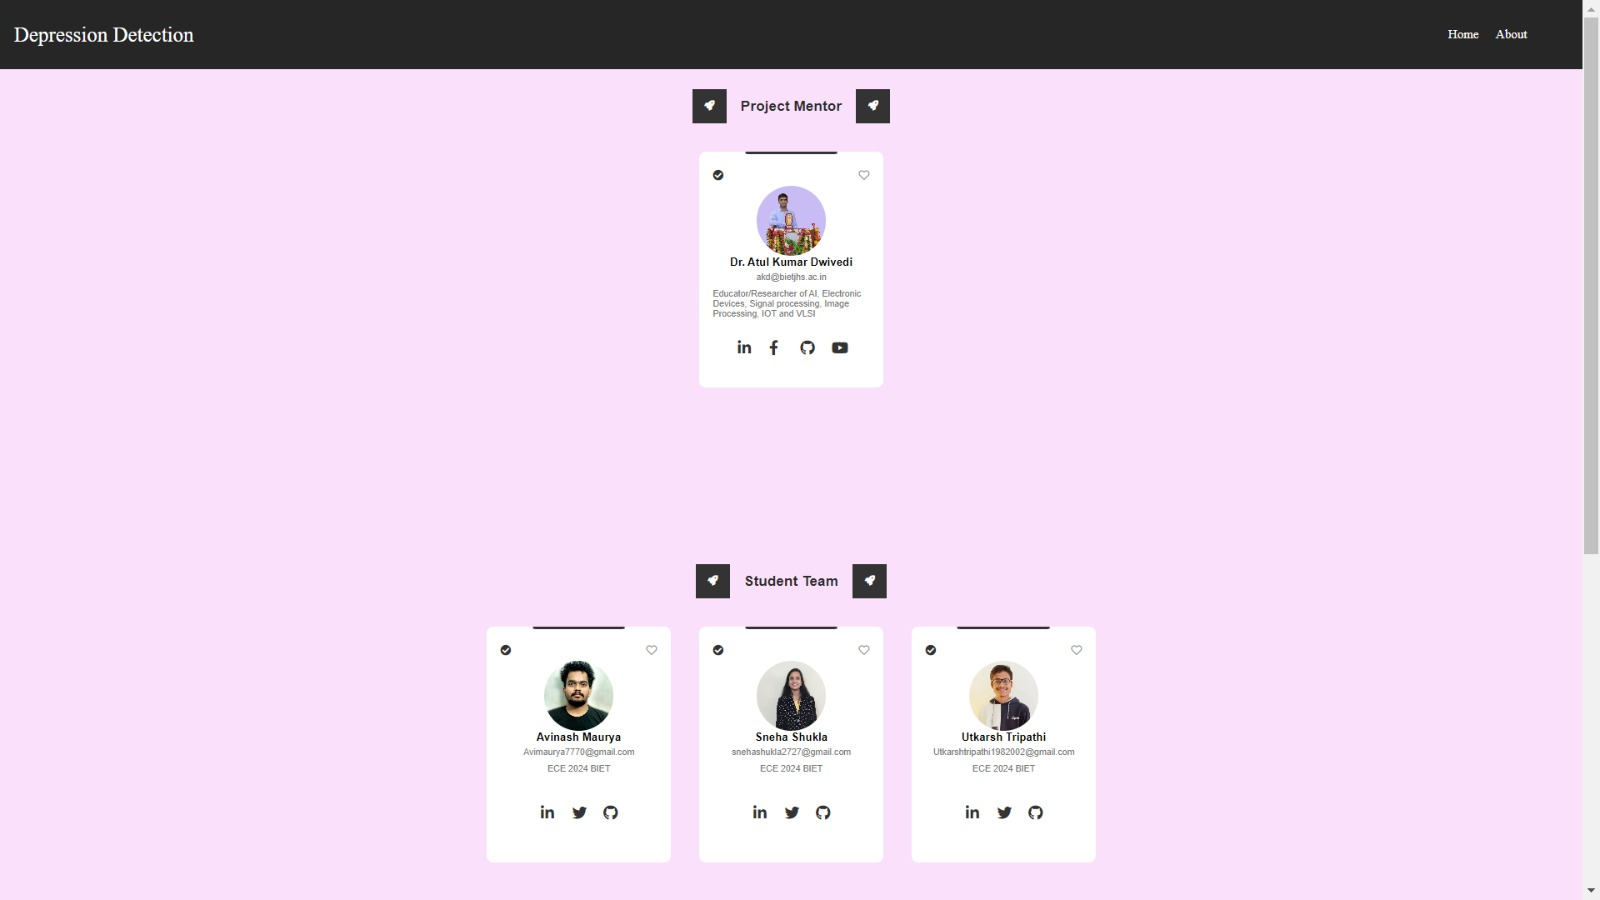
\includegraphics[width=1.0\linewidth]{C_chap/fig42.jpg}
\\\caption{About section of web page}
 \end{figure}
Our project's website serves as an interactive platform where users can assess and improve their mental well-being through the innovative application of machine learning. Upon visiting the site, users encounter a series of meticulously crafted questions designed to delve into various aspects of their emotional and mental health. These questions cover a wide range of topics, including mood fluctuations, energy levels, quality of sleep, patterns of social interaction, and more. Users provide their responses, which are then meticulously analyzed by sophisticated machine learning algorithms. Through this analysis, the platform generates personalized insights and guidance tailored to each user's unique mental health profile. These insights not only offer valuable self-awareness but also empower users to make informed decisions to enhance their overall well-being. Additionally, the platform may provide recommendations for further resources, such as articles, exercises, or professional support, based on the individual's responses and identified needs. By leveraging the power of machine learning, our platform aims to revolutionize mental health care, offering accessible, personalized support to users worldwide.
\\
Upon completing the questionnaire, users responses undergo thorough analysis by a machine learning model to ascertain their depression level. This analysis generates a score on a scale from 0 to 1, indicating varying degrees of depression severity. Scores falling between 0 and 0.15 denote severe depression, while those between 0.15 and 0.35 suggest moderate depression. A range of 0.35 to 0.65 indicates a neutral state, whereas scores from 0.65 to 0.85 signify a stable condition. Finally, a score between 0.85 and 1 represents an optimal mental state. This nuanced scoring system enables users to gain precise insights into their mental health status, guiding them towards appropriate interventions and support tailored to their individual needs.
\\
The web page provides users with a user-friendly platform to evaluate their mental health status independently and obtain personalized feedback through machine learning analysis. This streamlined approach offers individuals a convenient and accessible means to assess and track their mental well-being. By leveraging advanced algorithms, the platform delivers valuable insights and guidance tailored to each user's responses, empowering them to monitor and manage their mental health effectively. This innovative approach represents a significant step forward in mental health care, offering individuals the tools and support they need to prioritize their well-being in a proactive and informed manner.
\\
\pagebreak
\section{Result of Audio based Depression Detection}
The Convolution Neural Network (CNN) model implemented for audio-based depression detection exhibited a notable achievement with an accuracy of 82\% in correctly classifying individuals as either depressed or non-depressed based on acoustic features extracted from speech recordings. This accuracy signifies a promising step forward in leveraging machine learning techniques for mental health assessment. However, despite this moderate success, several avenues for enhancing the model's performance exist.
\\
 \begin{figure}[htbp]
    \centering
     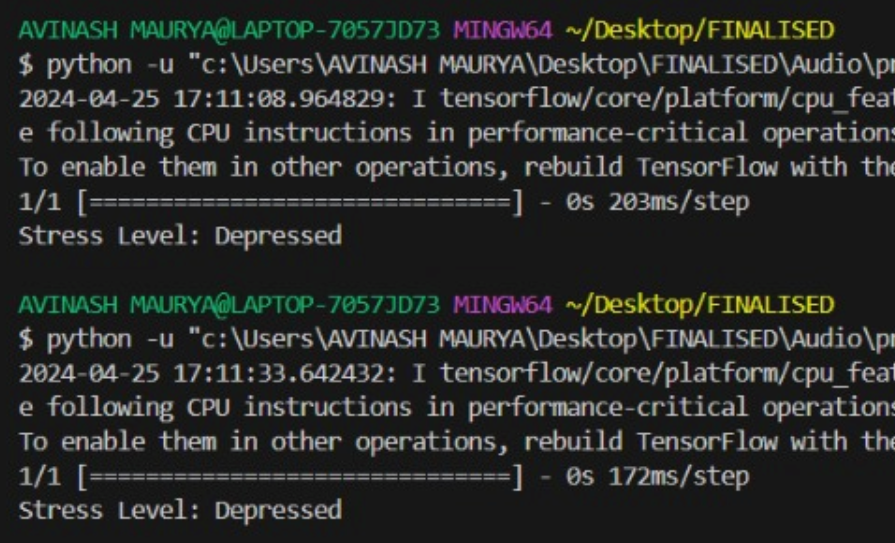
\includegraphics[width=0.8\linewidth]{C_chap/fig35.png}
\\\caption{Prediction of Audio Based Model}
 \end{figure}
\\
The Convolution Neural Network (CNN) model developed using TensorFlow and Keras libraries for audio classification achieved promising results. After thorough data processing, which involved extracting features like Mel-frequency cepstral coefficients (MFCCs) from audio files and augmenting the dataset with various techniques, the model was constructed with convolution and pooling layers followed by dense layers. During training, the model was put together using categorical cross-entropy loss and the Adam optimizer, achieving a significant accuracy rate. Evaluation on the test data yielded impressive metrics such as accuracy and F1 score, indicating the model's robustness in classifying emotions from audio recordings. The confusion matrix visualization further illustrated the model's performance, providing insights into its ability to accurately predict different emotional states. Overall, this comprehensive script showcases the effectiveness of deep learning techniques in audio classification tasks and highlights the potential for further advancements in this domain \cite{sardari2022audio}.
\\
 Firstly, refining the feature extraction process could involve delving deeper into the acoustic characteristics of speech that correlate with depression, potentially incorporating advanced signal processing techniques. Secondly, optimizing the network architecture might entail experimenting with different CNN configurations or exploring hybrid models that combine CNN with other types of feedforward networks. Moreover, augmenting the size and diversity of the training dataset could address potential biases and improve the model's robustness across various demographic groups. Additionally, while the 82\% accuracy suggests the model's potential utility, further research is warranted to validate its effectiveness in real-world clinical settings and to ascertain its specification across different populations, considering factors Including differences in age, gender, cultural background and language. This comprehensive evaluation is essential for ensuring the CNN model's reliability and practical applicability in supporting mental health diagnosis and intervention strategies.
\\
The CNN model demonstrated a 82\%  accuracy in discerning between depressed and non-depressed individuals using audio features from speech recordings, indicating a moderate level of effectiveness. However, there are opportunities for improvement in refining feature extraction, optimizing the network architecture, and enlarging the training dataset. Further research is necessary to evaluate the model's suitability across various populations and in clinical contexts. The figure provides a visual representation of how the CNN model categorizes individuals into depressed and non-depressed groups.